\section{Results}
\label{sec:results}

\para{Creative generation.} \Tabref{tab:generation-results} shows the full prompt-level comparison on \noveltybench. The only result that survives FDR correction is semantic spread: embedding dispersion rises from 0.803 to 0.831, with a moderate paired effect size ($d=0.73$). In contrast, the LN-free model slightly lowers \texttt{distinct\_1} and \texttt{distinct\_2}, slightly raises bigram overlap, and leaves repetition and sentence adherence effectively unchanged. The directional checks match this mixed picture. \lnfreegpt shows higher semantic dispersion on 15 of 20 prompts, but it beats \gpttwo on only 8 of 20 prompts for \texttt{distinct\_1} and 6 of 20 prompts for \texttt{distinct\_2}. \Figref{fig:generation-metrics} visualizes the same pattern: broader semantic spread without cleaner lexical novelty.

\begin{table*}[t]
\centering
\resizebox{\textwidth}{!}{%
\begin{tabular}{@{}lcccc@{}}
\toprule
\textbf{Metric} & \textbf{\gpttwo} & \textbf{\lnfreegpt} & \textbf{Delta (LN-free $-$ GPT-2)} & \textbf{FDR-adjusted $p$} \\
\midrule
\texttt{distinct\_1} & {\bf 0.463} [0.449, 0.476] & 0.451 [0.439, 0.464] & -0.0117 & 0.258 \\
\texttt{distinct\_2} & {\bf 0.899} [0.888, 0.909] & 0.884 [0.871, 0.896] & -0.0151 & 0.115 \\
\texttt{embedding\_dispersion} & 0.803 [0.772, 0.833] & {\bf 0.831} [0.804, 0.857] & +0.0285 & {\bf 0.024} \\
\texttt{pairwise\_bigram\_jaccard}$\downarrow$ & {\bf 0.0063} [0.0053, 0.0074] & 0.0081 [0.0067, 0.0096] & +0.0018 & 0.105 \\
\texttt{mean\_repetition\_rate}$\downarrow$ & 0.0277 [0.0170, 0.0404] & {\bf 0.0256} [0.0168, 0.0365] & -0.0021 & 0.766 \\
\texttt{sentence\_adherence} & {\bf 0.222} [0.167, 0.250] & 0.167 [0.083, 0.250] & -0.0556 & 0.600 \\
\bottomrule
\end{tabular}%
}
\caption{Creative-generation results on 20 \noveltybench prompts. Entries report mean with 95\% bootstrap confidence interval in brackets. For \texttt{pairwise\_bigram\_jaccard} and \texttt{mean\_repetition\_rate}, lower is better; higher is better for the other metrics. Best values are in \textbf{bold}.}
\label{tab:generation-results}
\end{table*}


\begin{figure}[t]
    \centering
    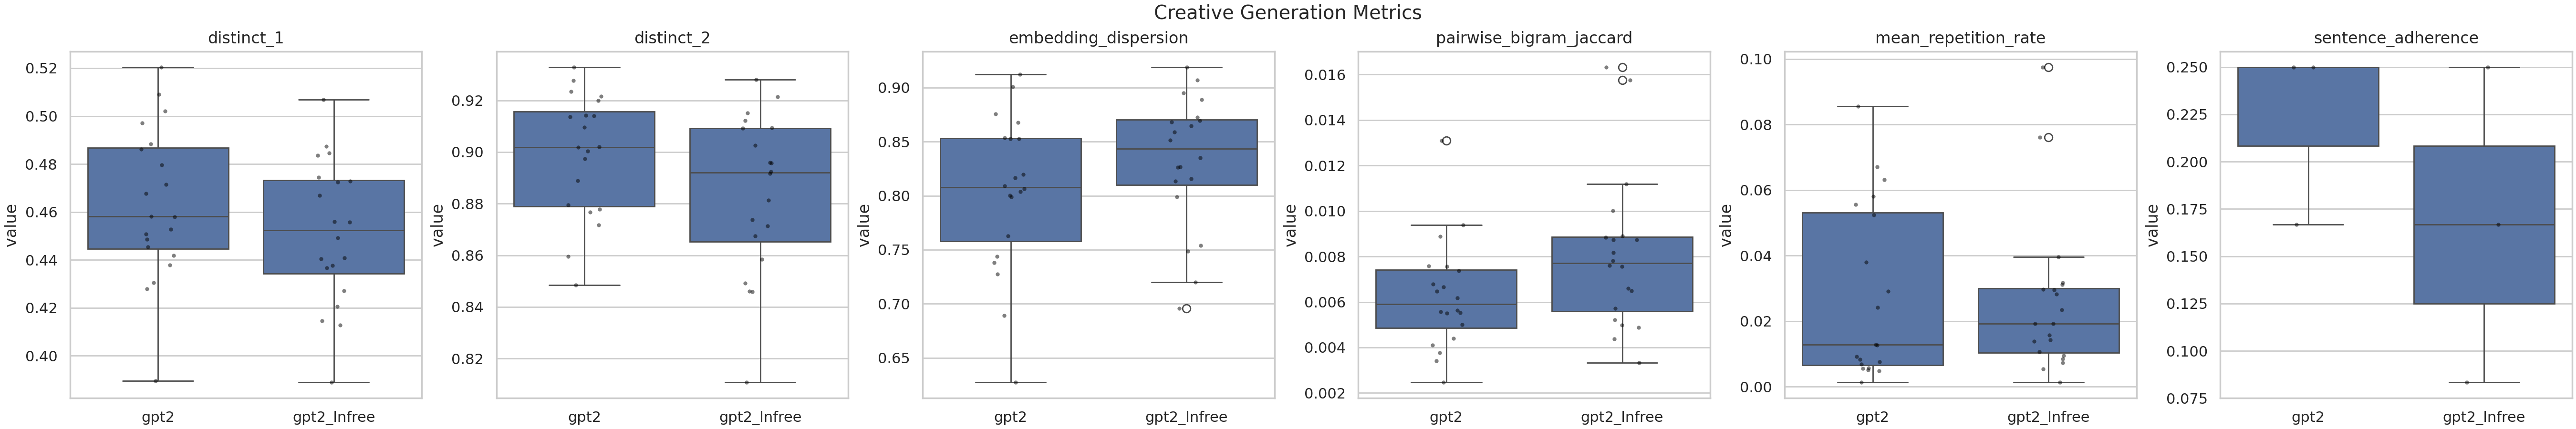
\includegraphics[width=0.95\linewidth]{figures/generation_metrics.png}
    \caption{Creative-generation metrics across 20 \noveltybench prompts. The LN-free model increases semantic dispersion, but the lexical metrics do not improve in parallel. This separation between semantic spread and surface distinctness is the central result on the generation side.}
    \label{fig:generation-metrics}
\end{figure}

\para{Association geometry.} \Tabref{tab:ocw-results} shows a much stronger effect on the \ocw benchmark. Removing LayerNorm does not significantly improve association AUC or similarity gap, but it changes embedding geometry substantially. Mean anisotropy falls from 0.992 to 0.964, and effective rank rises from 1.35 to 2.56. Both survive FDR correction by a large margin. The directional checks are even stronger: \lnfreegpt has lower anisotropy on all 62 walls and higher effective rank on all 62 walls. However, AUC improves on only 33 of 62 walls, which means the broader geometry does not translate into a reliable gain in clue-group separability.

\begin{table*}[t]
\centering
\resizebox{\textwidth}{!}{%
\begin{tabular}{@{}lcccc@{}}
\toprule
\textbf{Metric} & \textbf{\gpttwo} & \textbf{\lnfreegpt} & \textbf{Delta (LN-free $-$ GPT-2)} & \textbf{FDR-adjusted $p$} \\
\midrule
\texttt{association\_auc} & 0.527 [0.515, 0.540] & {\bf 0.529} [0.519, 0.541] & +0.0023 & 0.706 \\
\texttt{similarity\_gap} & 0.00058 [0.00031, 0.00089] & {\bf 0.00105} [0.00024, 0.00186] & +0.00047 & 0.299 \\
\texttt{anisotropy}$\downarrow$ & 0.992 [0.991, 0.992] & {\bf 0.964} [0.961, 0.967] & -0.0273 & {\bf $8.5\times10^{-26}$} \\
\texttt{effective\_rank} & 1.35 [1.27, 1.45] & {\bf 2.56} [2.35, 2.79] & +1.21 & {\bf $1.5\times10^{-11}$} \\
\bottomrule
\end{tabular}%
}
\caption{Association-geometry results on 62 \ocw validation walls. Entries report mean with 95\% bootstrap confidence interval in brackets. Lower anisotropy is better; higher is better for the remaining metrics. Best values are in \textbf{bold}.}
\label{tab:ocw-results}
\end{table*}


\begin{figure}[t]
    \centering
    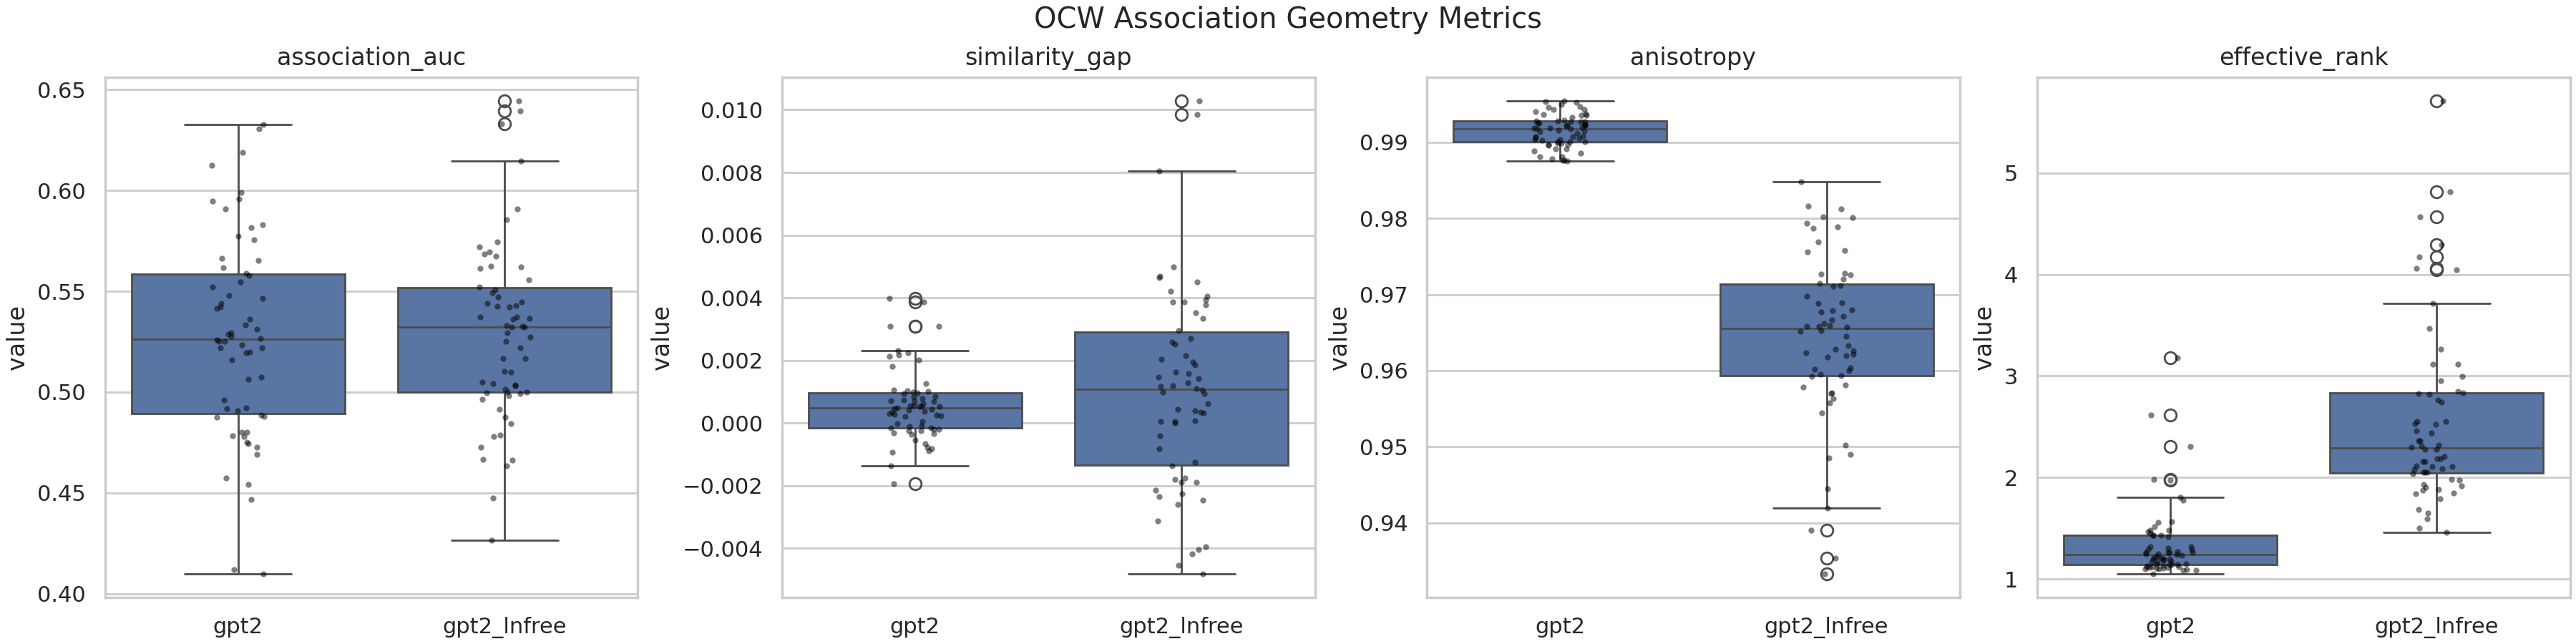
\includegraphics[width=0.95\linewidth]{figures/ocw_metrics.png}
    \caption{Association-geometry metrics across 62 \ocw validation walls. LN removal consistently lowers anisotropy and raises effective rank, but the separability metrics remain close to baseline. The figure highlights a strong internal change without a matching task-level gain.}
    \label{fig:ocw-metrics}
\end{figure}

\para{Statistical interpretation.} Taken together, the results support H2 strongly, support H1 only through semantic dispersion, and do not support H3 strongly enough to claim better association structure at the task level. The key empirical fact is therefore not a broad creativity gain, but a mismatch: LayerNorm removal expands representational geometry much more than it improves surface behavior.
